%%%%%%%%%%%%%%%%%%%%%%%%%%%%%%%%%%%%%%%%%%%%%%%%%%%%%%%%%%%%%%%%%%%%%%%
% BAB 5
%%%%%%%%%%%%%%%%%%%%%%%%%%%%%%%%%%%%%%%%%%%%%%%%%%%%%%%%%%%%%%%%%%%%%%%

\mychapter{5}{BAB 5 PERANCANGAN DAN IMPLEMENTASI}

\section{Perancangan Sistem}

Tahapan perancangan sistem merupakan sebuah tahapan yang dilakukan
setelah selesainya proses rekayasa kebutuhan. Hasil tahapan
perancangan nantinya digunakan sebagai landasan tahapan implementasi
sistem. Tiga bagian yang terdapat pada tahapan ini adalah
perancangan arsitektur, perancangan komponen, dan perancangan
antarmuka.

\subsection{Perancangan Arsitektur}

Sistem dibangun menggunakan arsitektur \emph{Model-View-Controller (MVC)}.
Maka komponen fungsionalitas inti sistem terpisah dari komponen antarmuka
sistem. Pemisahan ini memberikan manfaat untuk pengembangan sistem pada tahap
selanjutnya. Salah satu manfaat tersebut adalah kemudahan dalam mengembangkan
antarmuka lain untuk sistem, hal ini dikarenakan pengembang hanya fokus pada
komponen antarmuka yang akan dibangun.
Perancangan arsitektur dilakukan dengan menggunakan notasi \emph{UML}
\emph{sequence diagram} dan \emph{class diagram}. \emph{Class diagram}
bertujuan menggambarkan struktur sistem dan relasi antar komponen dalam sistem
secara statis. Pada \emph{class diagram} digambarkan \emph{class},
\emph{method} atau
\emph{function}, dan relasi antar \emph{class}. \emph{Sequence
  diagram} merupakan diagram dinamis yang berfungsi untuk
menggambarkan interaksi antar komponen atau objek yang berada di dalam sistem.
Terdapat tiga sampel \emph{sequence diagram} yang akan dipaparkan pada
bagian ini. Tiga sampel tersebut adalah \emph{sequence diagram} untuk
merekam pengerjaan tugas, \emph{sequence diagram} untuk melihat hasil
rekaman, dan \emph{sequence diagram} untuk melihat grafik \emph{edit-distance}
tugas sebelumnya. Sementara itu, \emph{class diagram} sistem akan dipaparkan seluruhnya.

\subsubsection{\emph{Sequence Diagram} Merekam Pengerjaan Tugas}

\emph{Sequence diagram} untuk merekam pengerjaan tugas dapat
dilihat pada Gambar~\ref{fig:sd-record}. Pada \emph{sequence diagram}
tersebut terdapat beberapa objek yang berinteraksi. Satu objek
\emph{boundary} ``\emph{MainView}'', dua objek \emph{controller}
``\emph{Controller}'' dan ``\emph{RecordWorker}'', dan satu objek
\emph{entity} ``\emph{Model}''. Aktor yang terlibat adalah mahasiswa.

\subsubsection{\emph{Sequence Diagram} Melihat Hasil Rekaman}

\emph{Sequence diagram} untuk melihat hasil rekaman dapat
dilihat pada Gambar~\ref{fig:sd-view-record-result}. Pada \emph{sequence diagram}
tersebut terdapat beberapa objek yang berinteraksi. Dua objek
\emph{boundary} ``\emph{MainView}'' dan ``\emph{LogView}'', dua objek \emph{controller}
``\emph{LogController}'' dan ``\emph{MainController}'', dan satu objek
\emph{entity} ``\emph{LogModel}''. Aktor yang terlibat adalah dosen.

\subsubsection{\emph{Sequence Diagram} Melihat Grafik \emph{Edit-Distance} Tugas Sebelumnya}

\emph{Sequence diagram} untuk melihat grafik \emph{edit-distance} tugas
sebelumnya dapat dilihat pada Gambar~\ref{fig:sd-view-previous-ed}.
Pada \emph{sequence diagram} tersebut terdapat beberapa objek yang
berinteraksi. Satu objek \emph{boundary} ``\emph{SearchView}'', satu objek
\emph{controller} ``\emph{SearchController}'', dan dua objek \emph{entity}
``\emph{SearchModel}'' dan ``\emph{MainModel}''. Aktor yang terlibat adalah dosen.

\begin{figure}[tph]
  \centering
  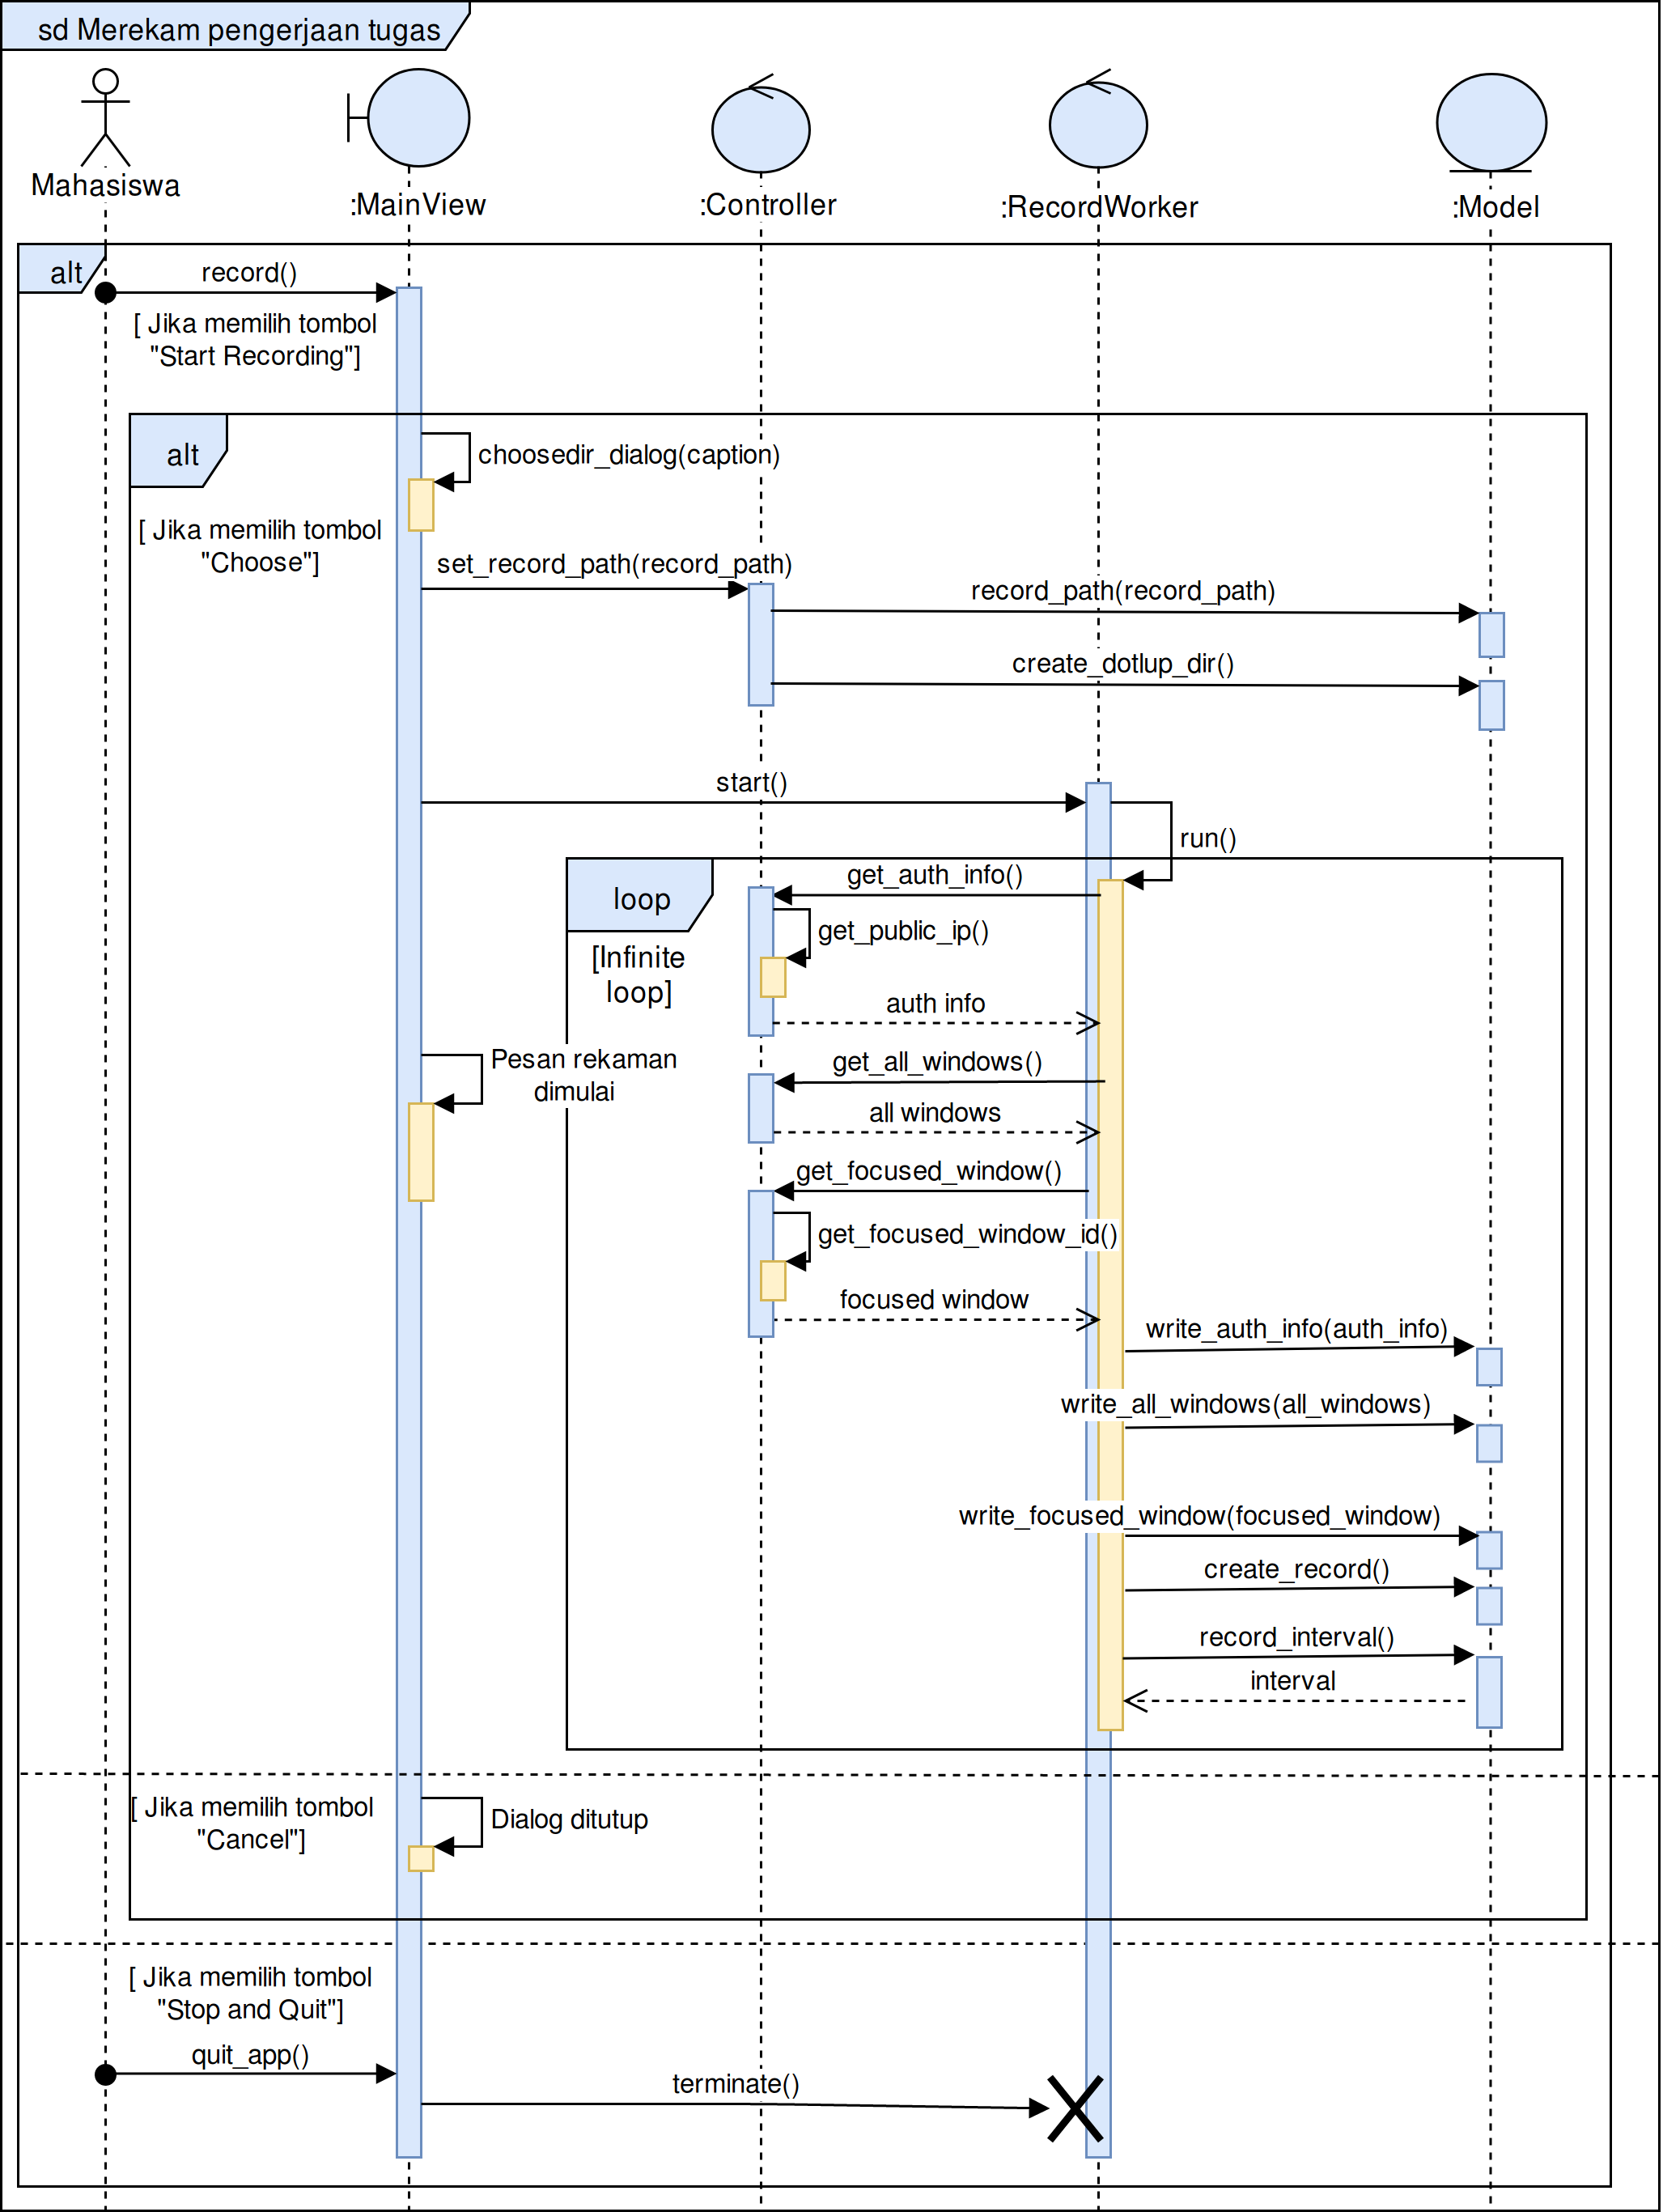
\includegraphics[width=.9\linewidth]{img/use-case/sd/sd-record-v2_4}
  \caption{\emph{Sequence diagram} Merekam Pengerjaan Tugas}\label{fig:sd-record}
\end{figure}

\begin{figure}[tph]
  \centering
  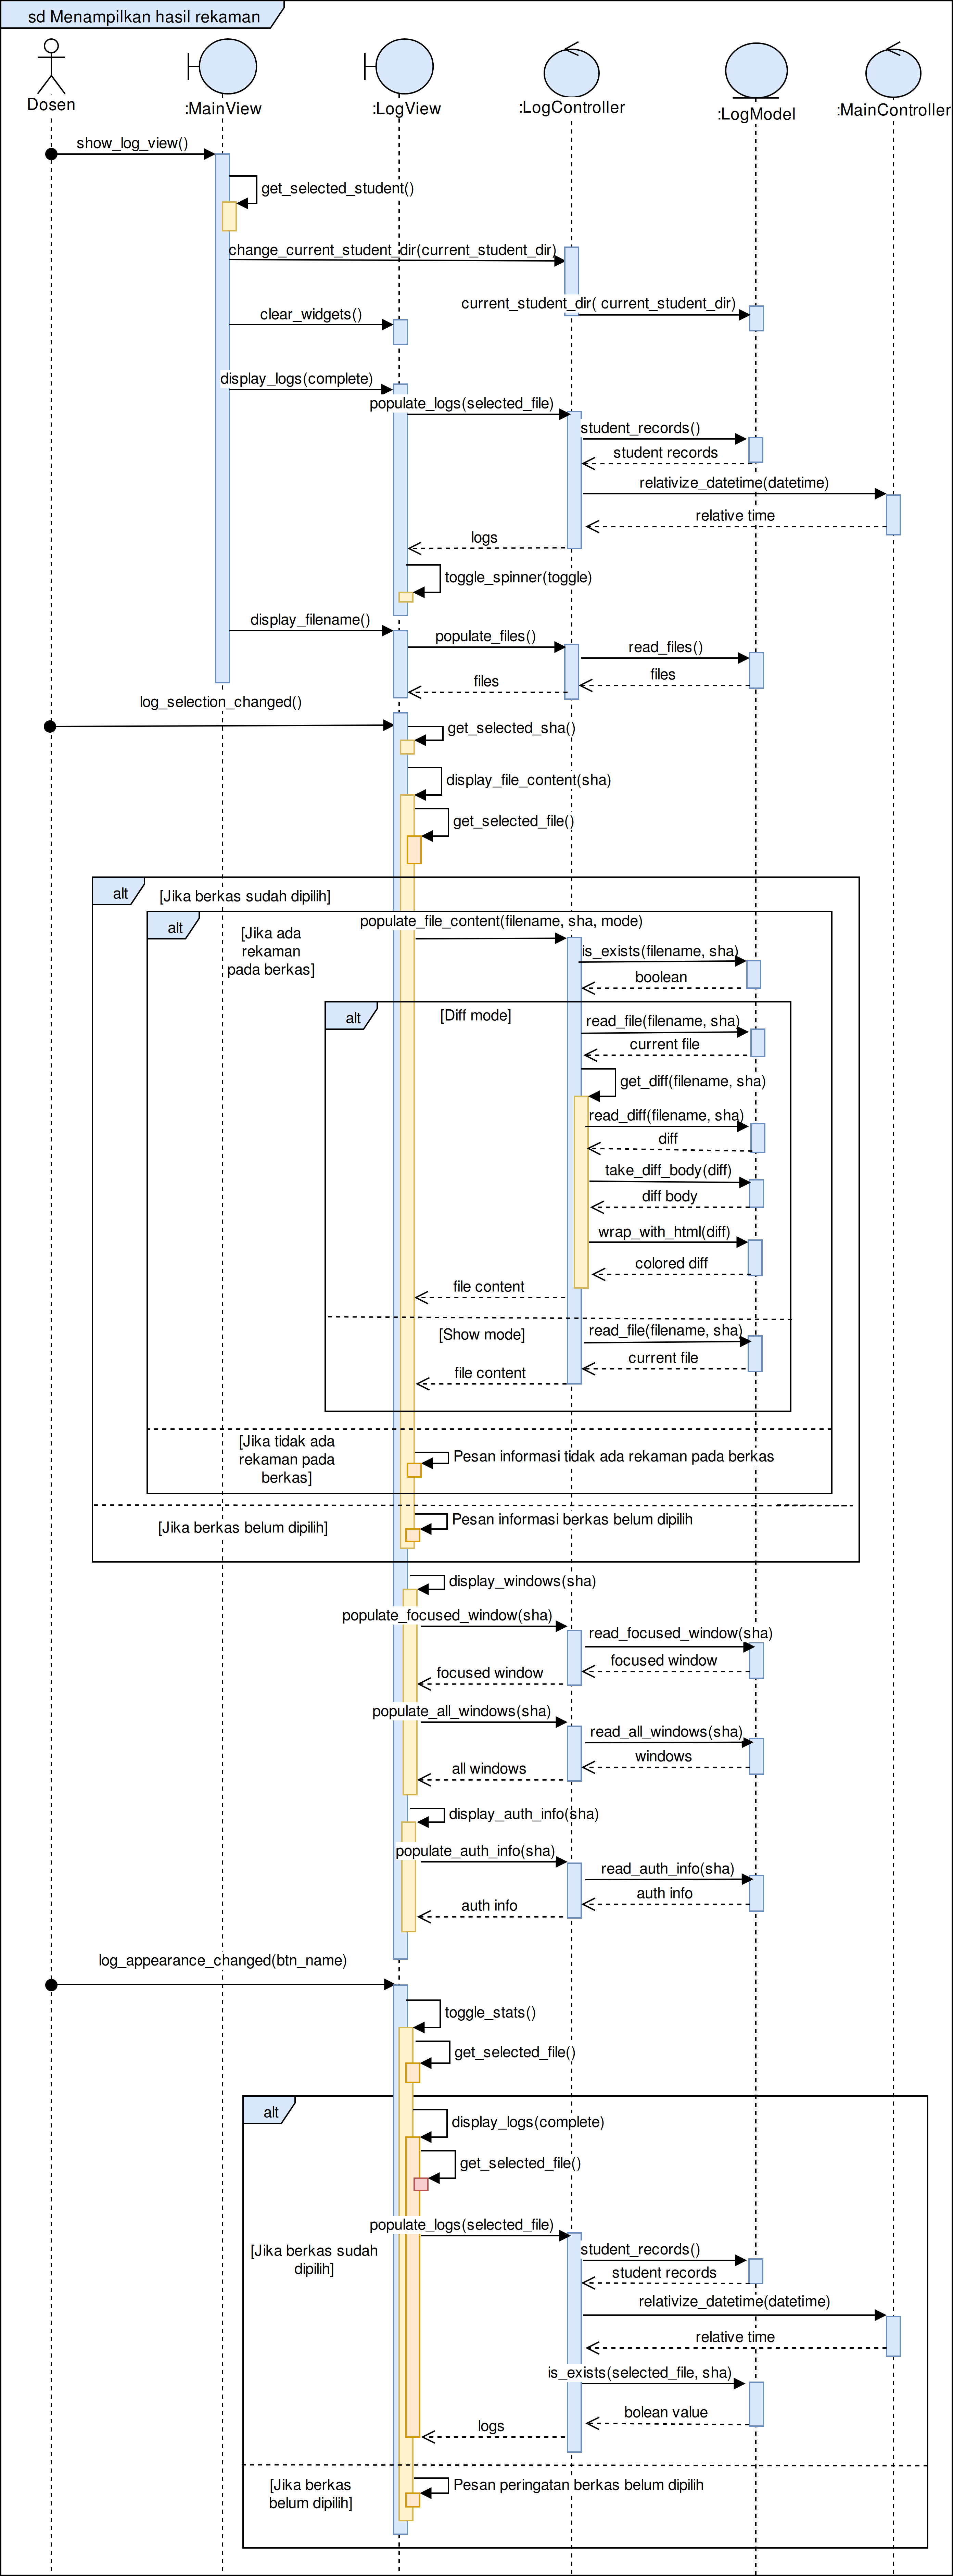
\includegraphics[width=.6\linewidth]{img/use-case/sd/sd-view-record-result-v1}
  \caption{\emph{Sequence diagram} Melihat Hasil Rekaman}\label{fig:sd-view-record-result}
\end{figure}

\begin{figure}[tph]
  \centering
  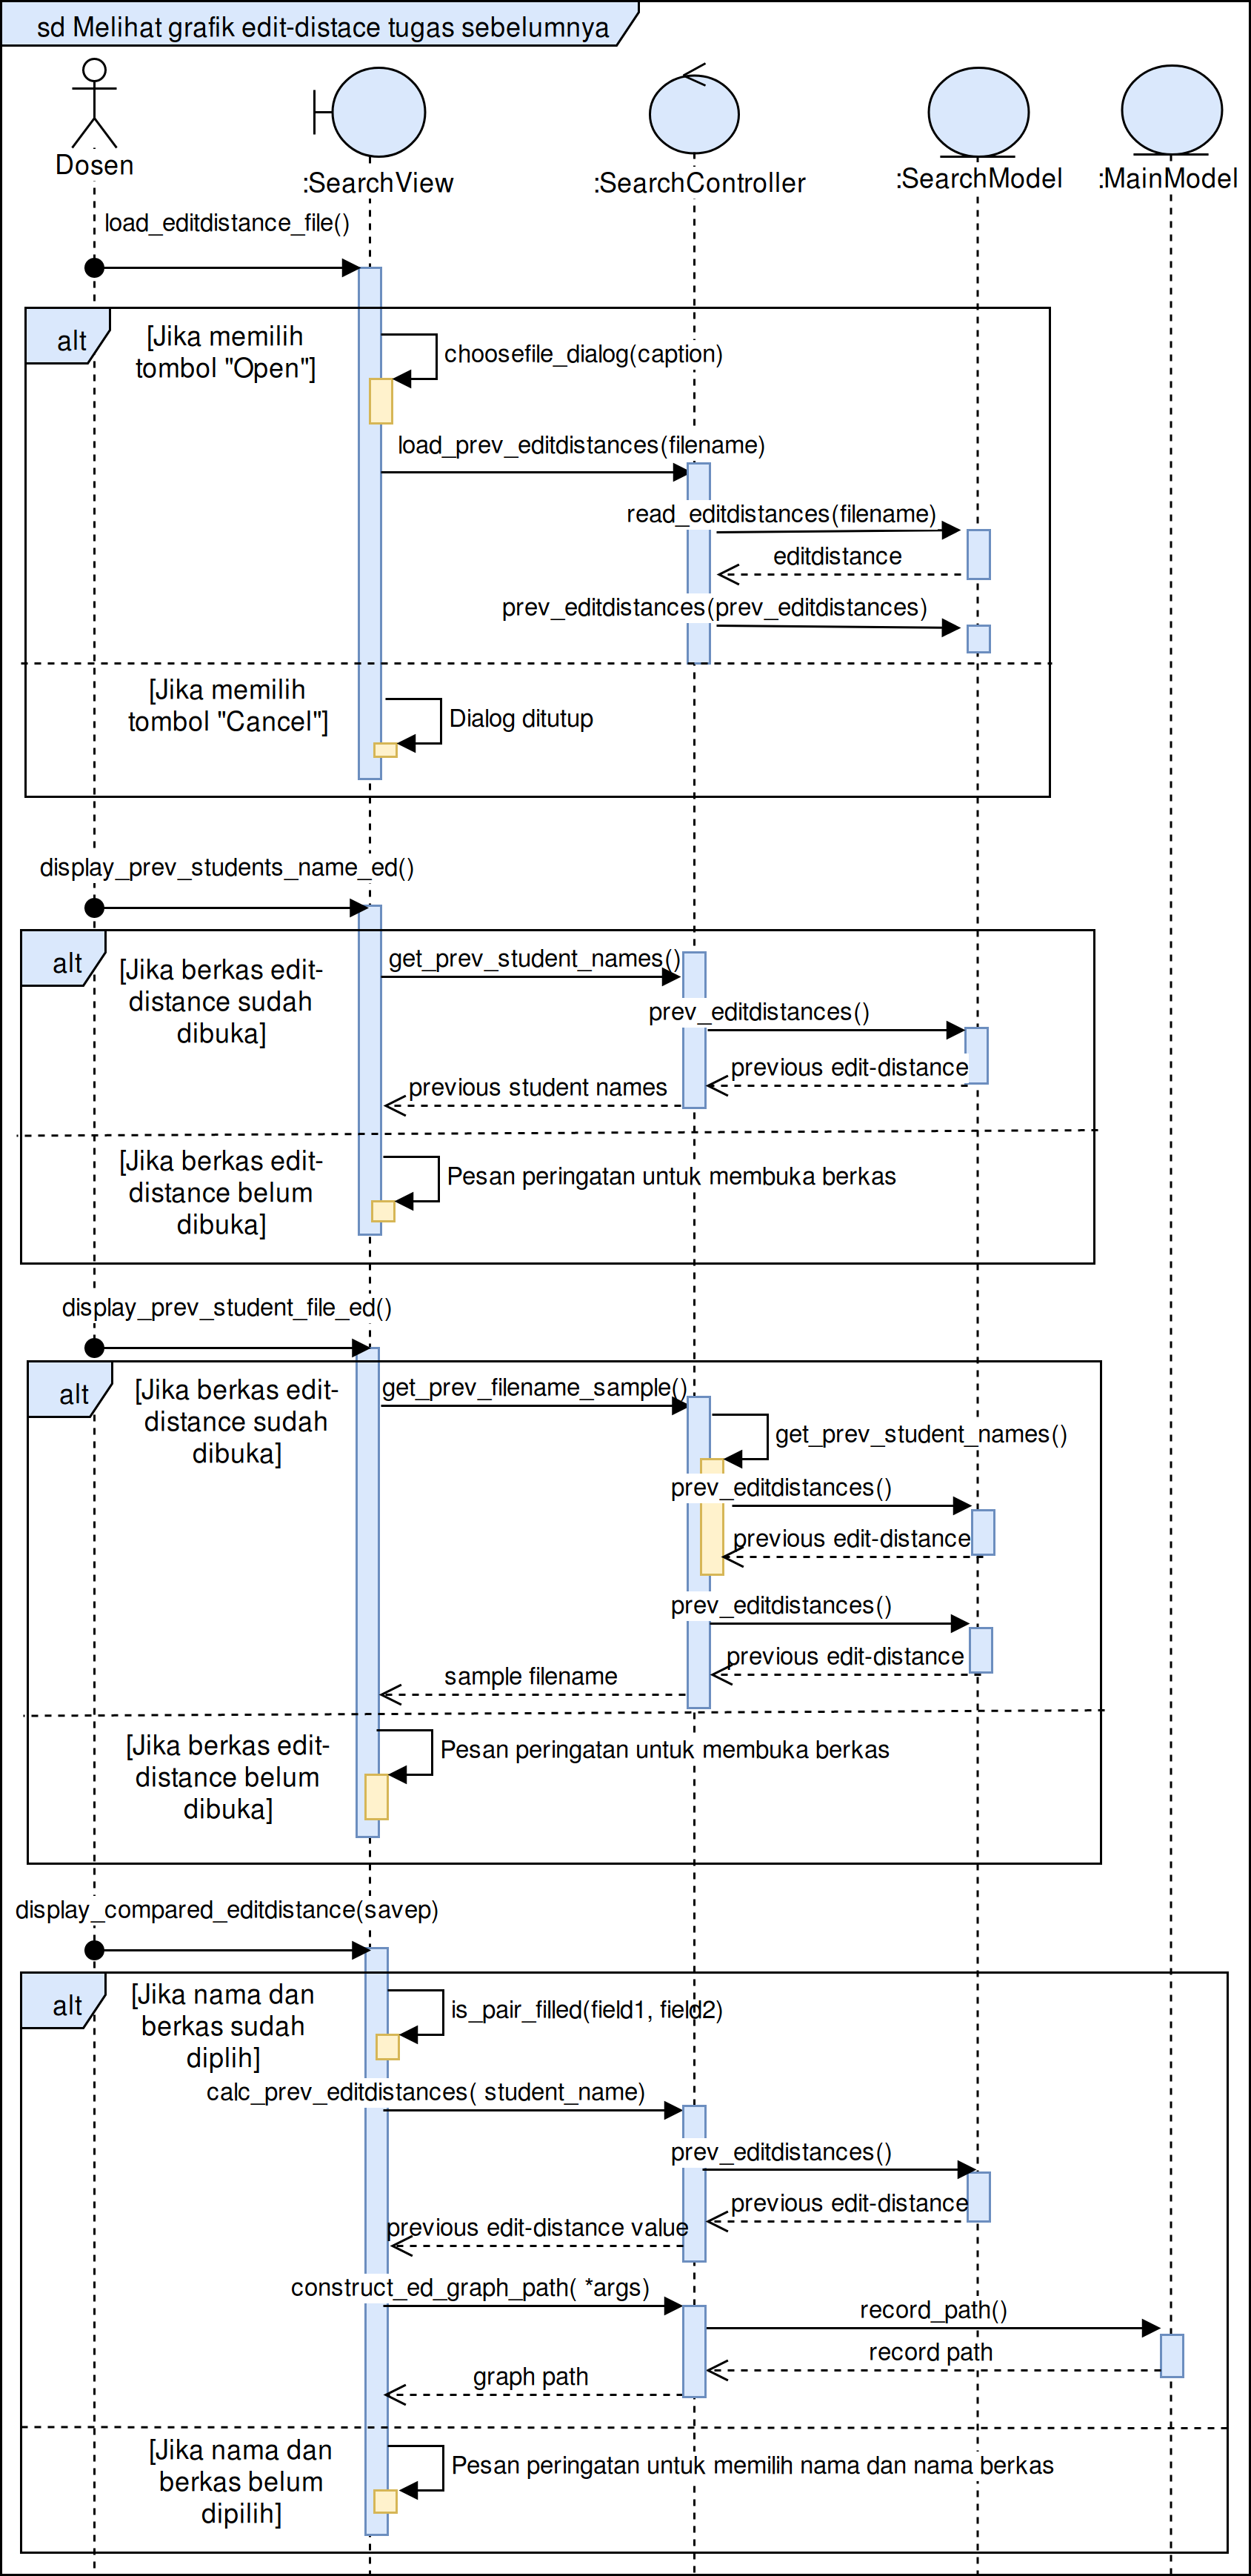
\includegraphics[width=.8\linewidth]{img/use-case/sd/sd-view-previous-ed-v1_2}
  \caption{\emph{Sequence diagram} Melihat Grafik \emph{Edit-Distance} Tugas
    Sebelumnya}\label{fig:sd-view-previous-ed}
\end{figure}

\subsubsection{\emph{Class Diagram}}

Pada bagian ini akan dipaparkan \emph{class}-\emph{class} yang menyusun sistem yang
dibangun. Gambar~\ref{fig:class-lupr} merupakan \emph{class diagram}
dari sistem \emph{Lup Recorder}, dan Gambar~\ref{fig:class-lupv}
merupakan \emph{class diagram} dari sistem \emph{Lup Viewer}. Sistem
yang dibangun menggunakan arsitektur \emph{Model-View-Controller}
sehingga \emph{class}-\emph{class} yang menyusun sistem pada \emph{class diagram}
umumnya terdiri dari \emph{class} \emph{Model}, \emph{class} \emph{View} dan \emph{class}
\emph{Controller}. Pada \emph{class diagram} juga dipaparkan relasi
antar \emph{class} yang umumnya merupakan relasi agregasi dan komposisi.

\begin{figure}[tph]
  \centering
  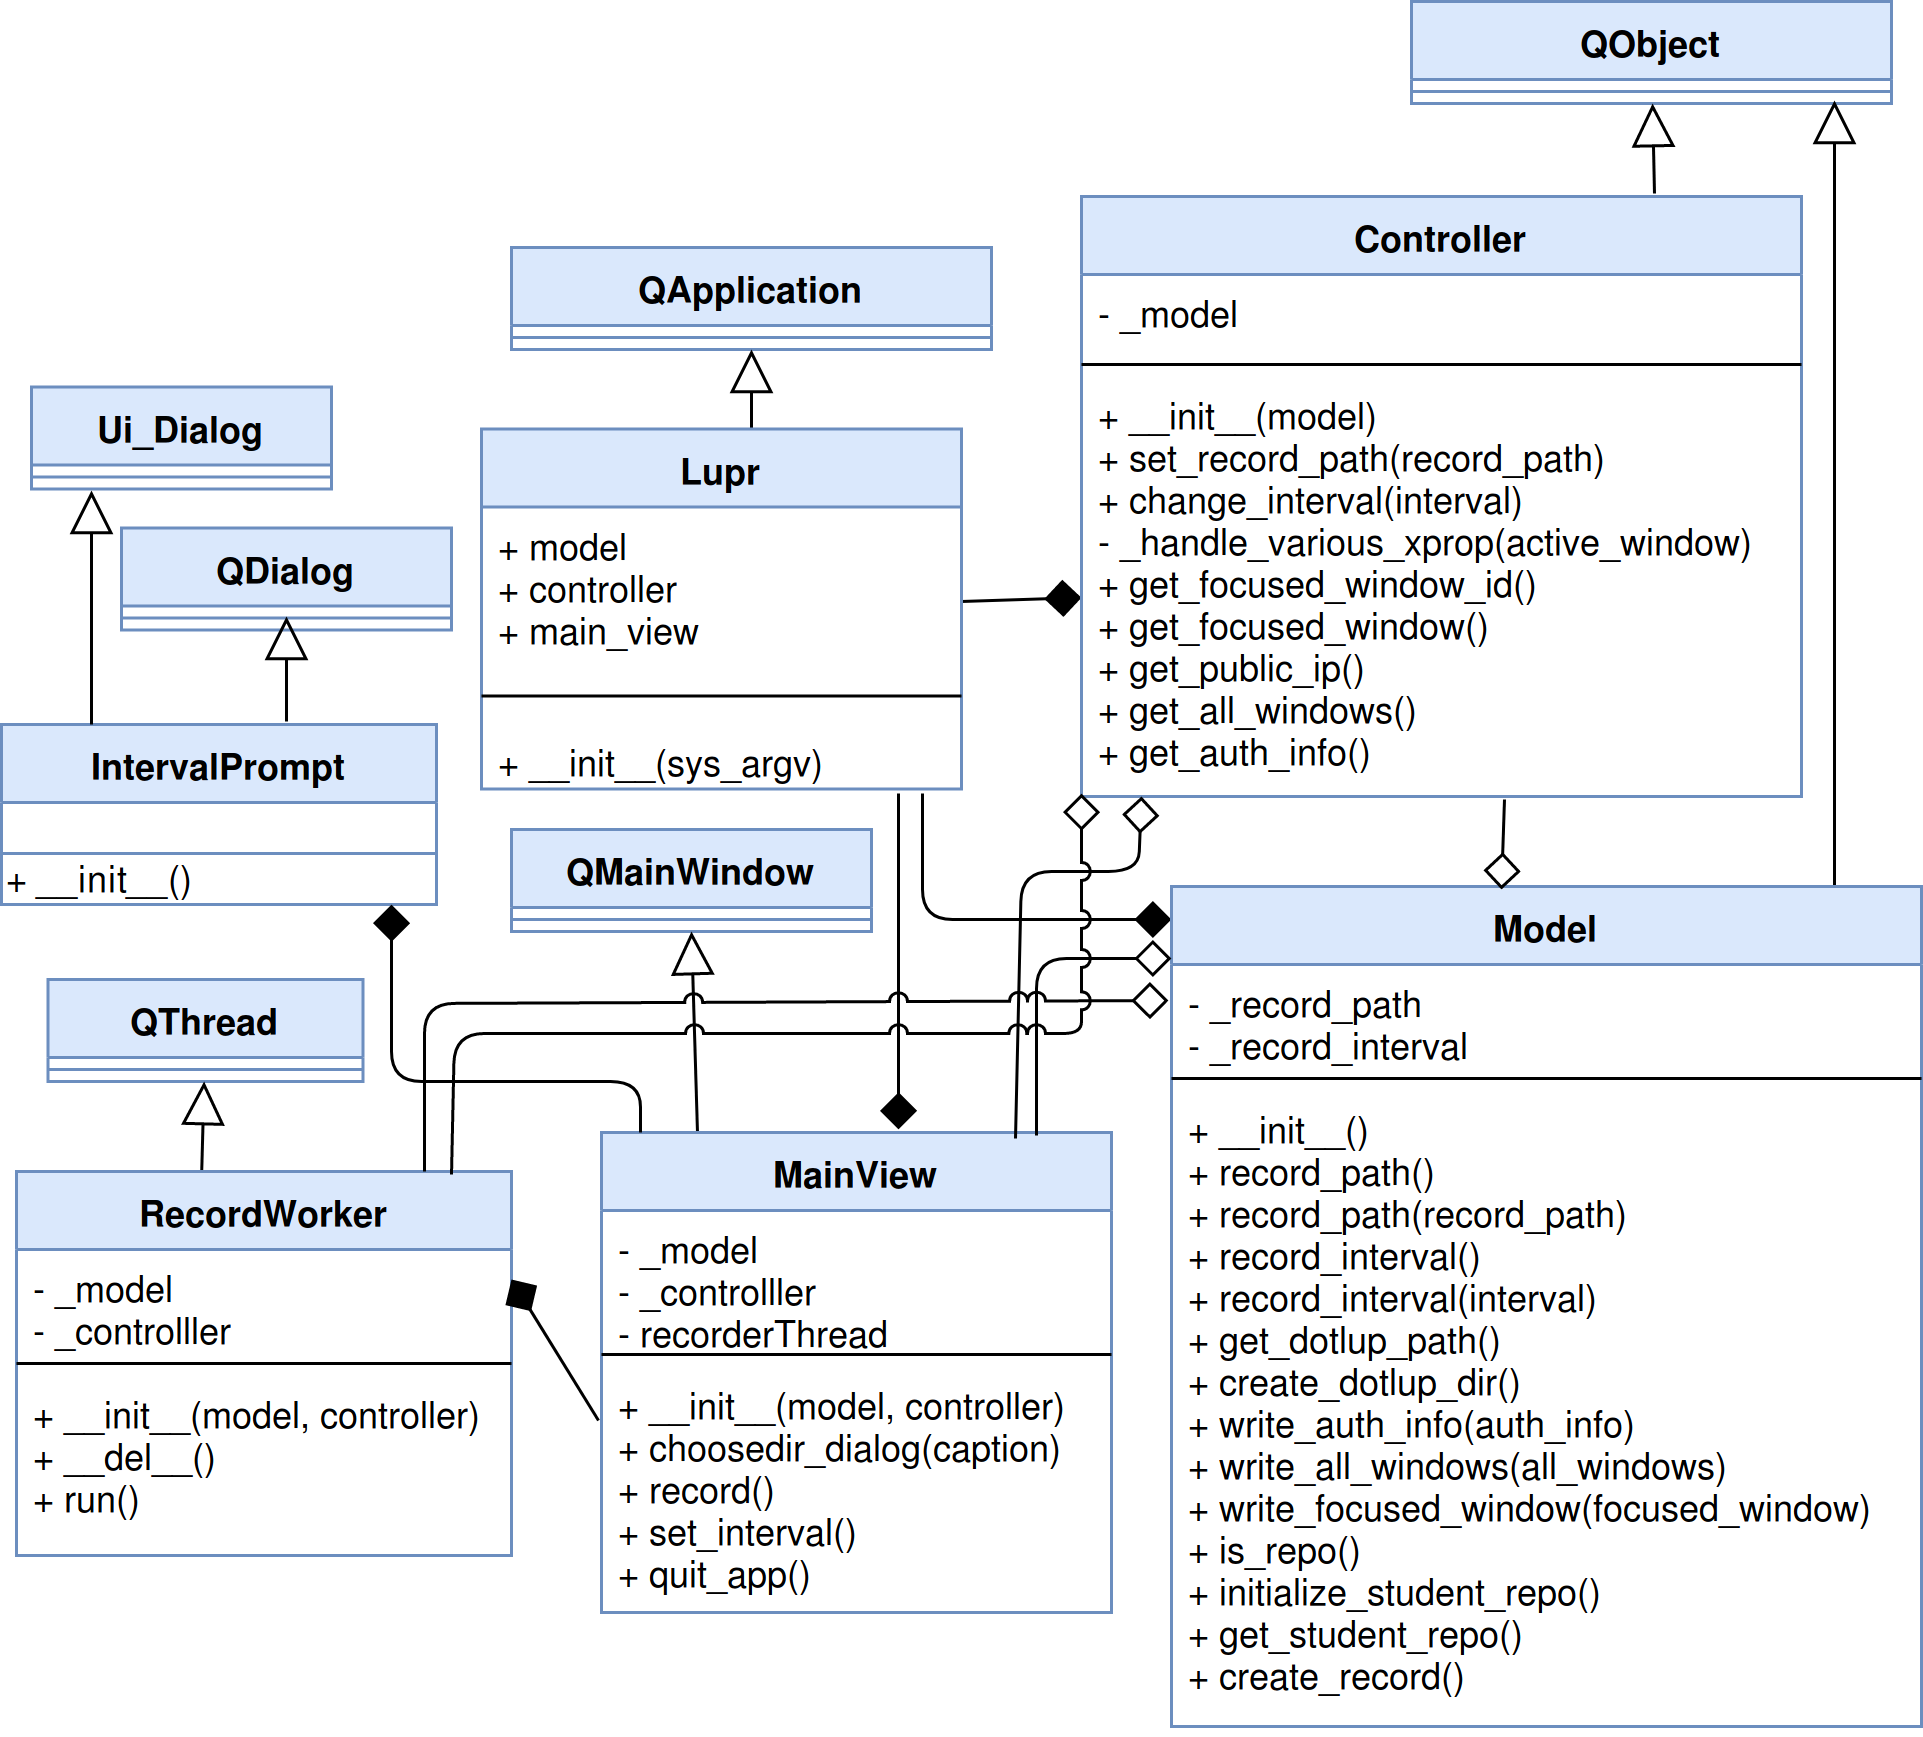
\includegraphics[width=.9\linewidth]{img/use-case/cd/class-lupr-v1_4}
  \caption{Pemodelan \emph{class diagram} \emph{Lup Recorder}}\label{fig:class-lupr}
\end{figure}

\begin{figure}[tph]
  \centering
  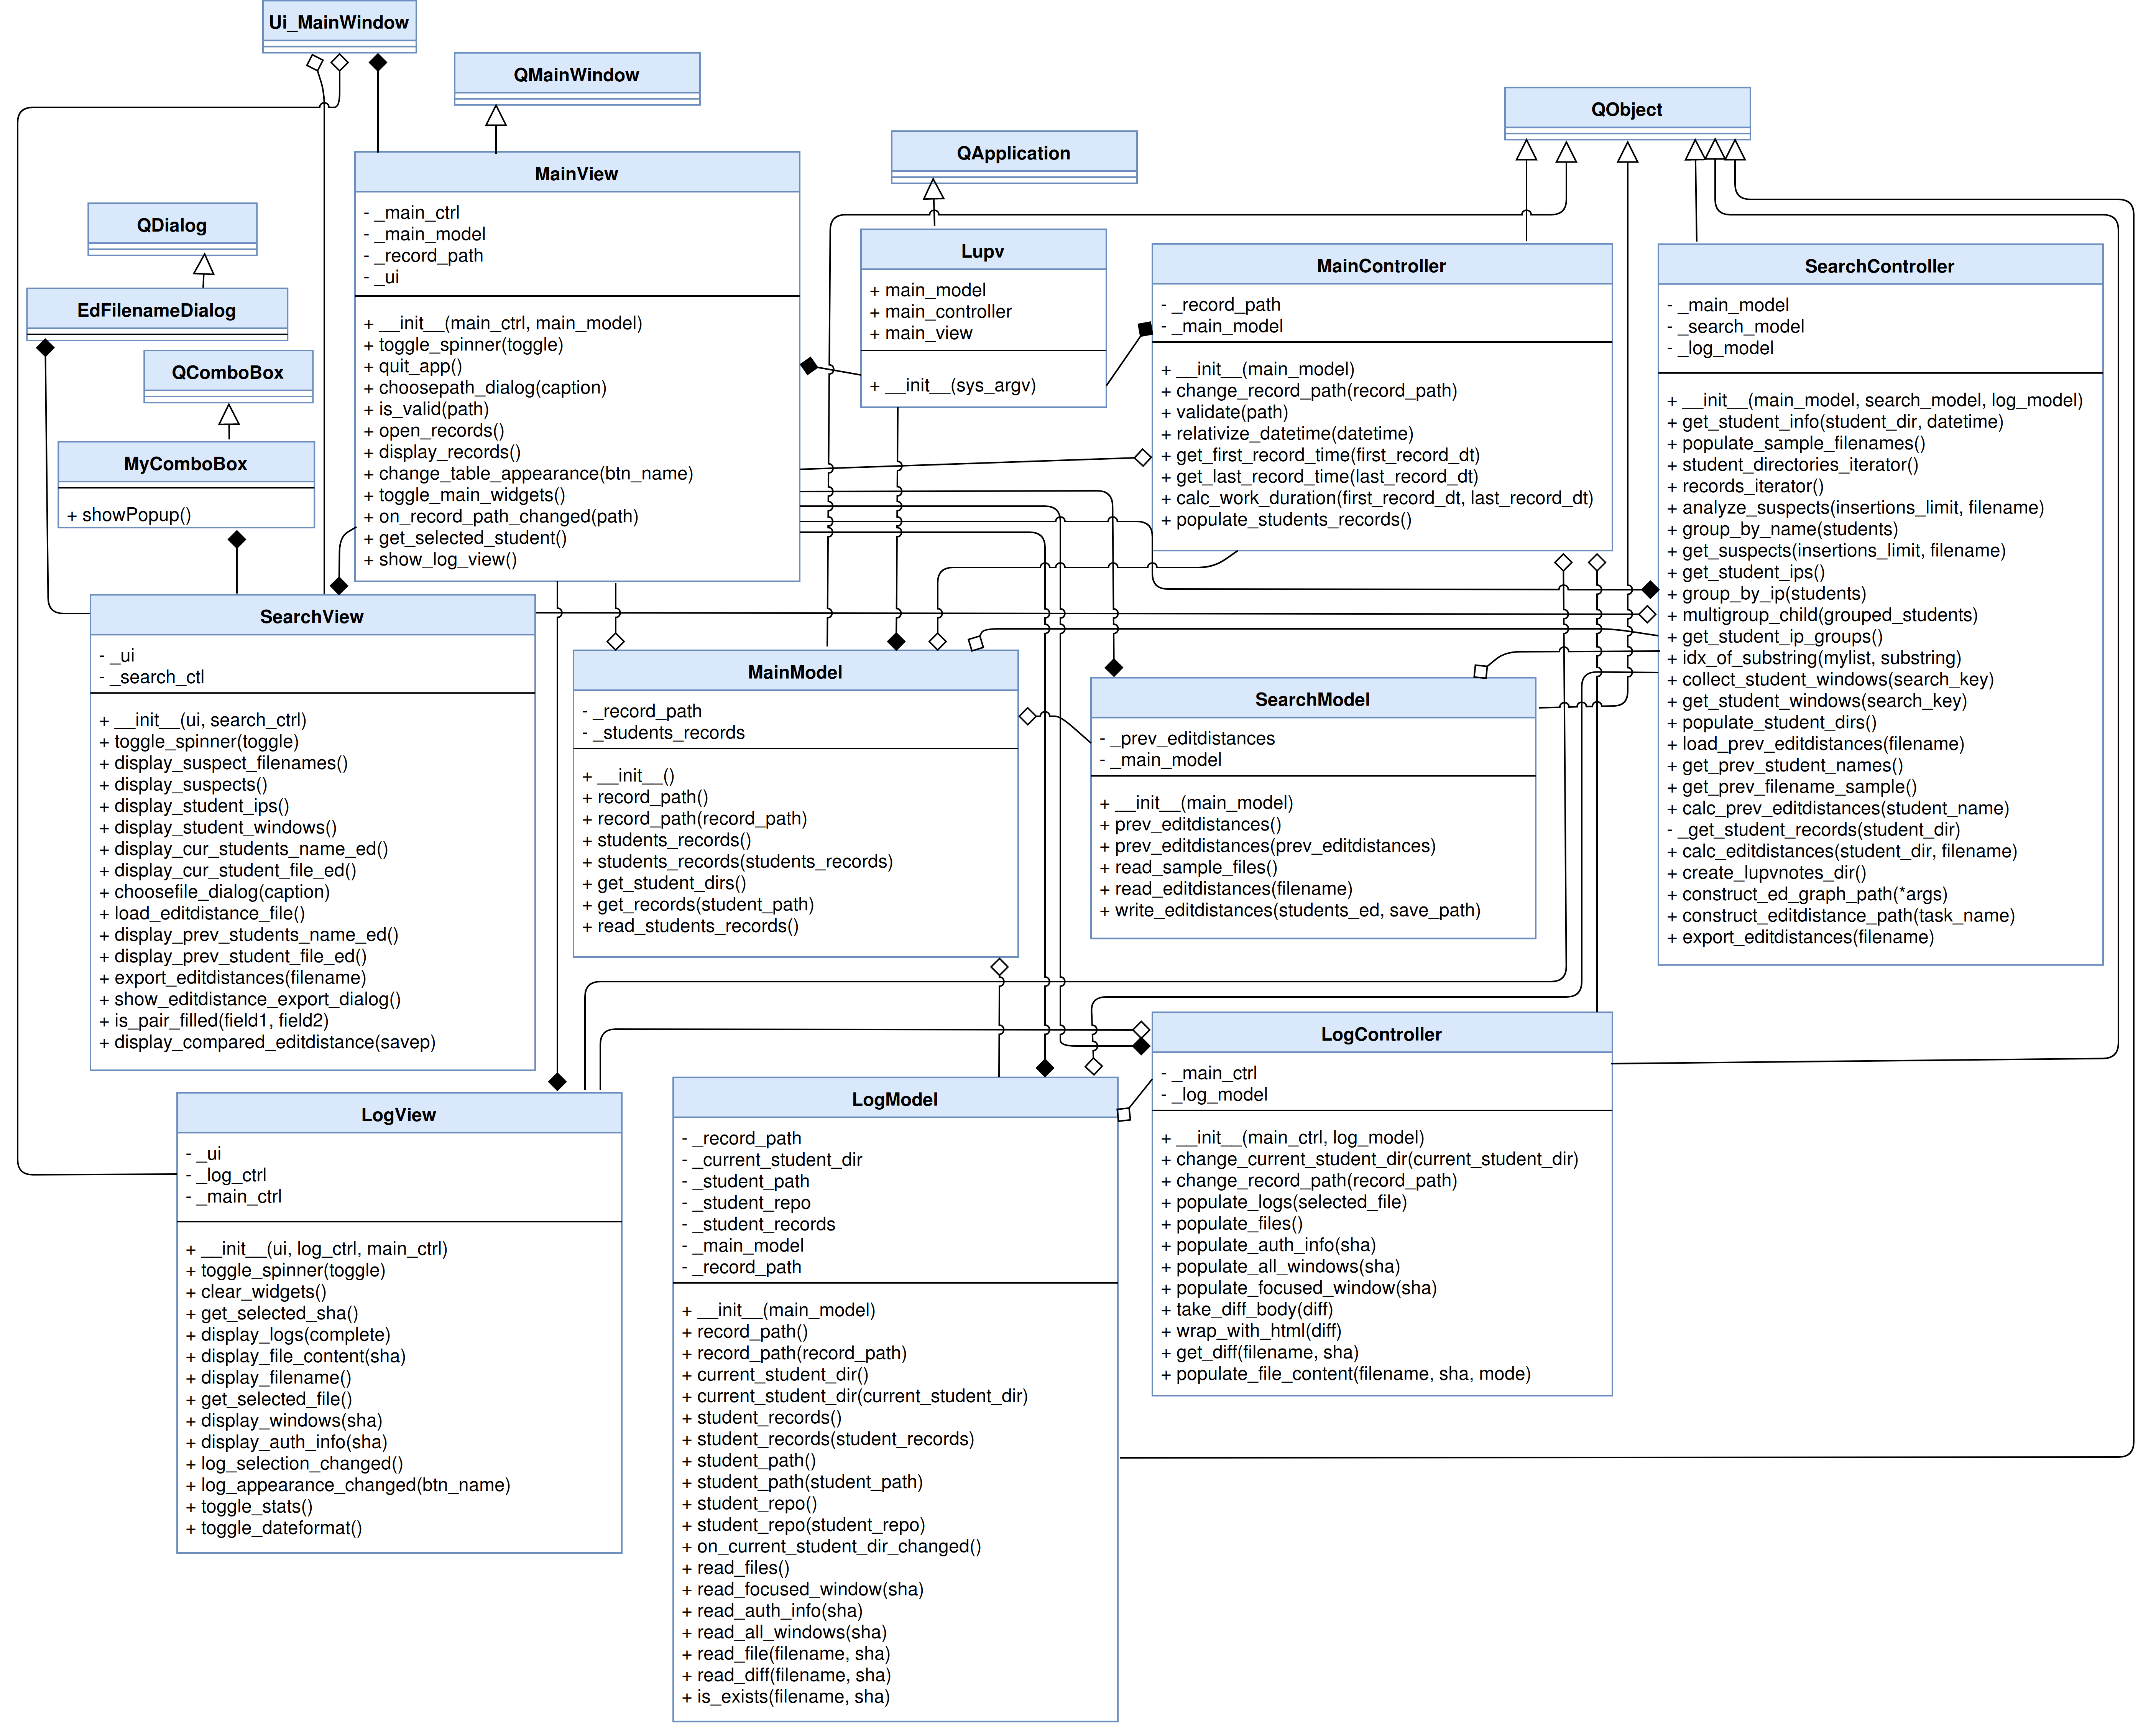
\includegraphics[angle=90,width=1.1\linewidth]{img/use-case/cd/class-lupv-v1_4}
  \caption{Pemodelan \emph{class diagram} \emph{Lup Viewer}}\label{fig:class-lupv}
\end{figure}

\subsection{Perancangan Komponen}

Pada tahapan perancangan komponen, komponen-komponen yang membentuk
sistem akan dirancang menggunakan \emph{pseudocode}. Komponen yang
membentuk sistem dalam sistem berorientasi objek adalah \emph{class}. Maka
tahapan ini akan memaparkan perancangan tiga sampel \emph{class}. Tidak semua
\emph{procedure} atau \emph{function} di dalam suatu \emph{class} akan
dipaparkan, melainkan hanya satu sampel \emph{function} dari tiap-tiap
\emph{class}. Tabel Kode~\ref{pc:get_all_windows} memaparkan \emph{pseudocode} untuk \emph{function}
\emph{get\_all\_windows} dari \emph{class} \emph{Controller} pada sistem \emph{Lup
  Recorder}. Tabel Kode~\ref{pc:populate_logs} memaparkan \emph{pseudocode} untuk
\emph{function} \emph{populate\_logs} dari \emph{class} \emph{LogController} pada
sistem \emph{Lup Viewer} dan, Tabel Kode~\ref{pc:construct-graph-path} memaparkan
\emph{pseudocode} untuk \emph{function} \emph{construct\_ed\_graph\_path}
dari \emph{class} \emph{SearchController} pada sistem \emph{Lup Viewer}.

\subsubsection{Perancangan Komponen \emph{Class} \emph{Controller}}

Pada Tabel Kode~\ref{pc:get_all_windows} dipaparkan \emph{pseudocode}
\emph{get\_all\_windows} pada sistem \emph{Lup
  Recorder}. \emph{Pseudocode} \emph{get\_all\_windows} dirancang
untuk membaca seluruh \emph{window} yang sedang dibuka. Sistem operasi
memiliki banyak atribut selain nama \emph{window}, maka
\emph{get\_all\_windows} hanya mengambil nilai nama \emph{window} dan
mengembalikannya.

\par\null\par
\begin{code}
\begin{ignasicblock}[title=get\_all\_windows,minted language=text]
START
  READ all_windows_dirty
  IF all_windows_dirty is true
    SET all_windows_dirty to split every line
    FOR each window in all_windows_dirty
      GET window_name
      SET all_windows = window_name
    ENDFOR
  ENDIF
  RETURN all_windows
END
\end{ignasicblock}
    \captionof{listing}{\emph{Pseudocode function get\_all\_windows}}\label{pc:get_all_windows}
\end{code}

\subsubsection{Perancangan Komponen \emph{Class} \emph{LogController}}

Pada Tabel Kode~\ref{pc:populate_logs} dipaparkan \emph{pseudocode}
\emph{populate\_log} pada sistem \emph{Lup Viewer}. \emph{Pseudocode}
\emph{populate\_log} dirancang untuk membaca seluruh rekaman
mahasiswa, dari setiap rekaman diambil nilai-nilai yang dibutuhkan
di antaranya adalah waktu rekaman, baris yang ditambah, dan baris yang
dihapus.

\par\null\par
\begin{code}
\begin{ignasicblock}[title=populate\_logs,minted language=text]
START
  CALL log_model RETURNING student_records

  FOR each record in student_records
    CALL main_ctrl with relativize_datetime RETURNING relative_time
    GET time
    GET sha
    SET insetion to 0
    SET deletion to 0
    IF selected_file is true
      IF CALL log_model with is_exist RETURNING true
        GET insertion
        GET deletion
      ENDIF
    ENDIF
  ENDFOR
  SET log to (relative_time, time, sha, insertion, deletion)
  RETURN log
END
\end{ignasicblock}
  \captionof{listing}{\emph{Pseudocode function} \emph{populate\_logs}}\label{pc:populate_logs}
\end{code}

\subsubsection{Perancangan Komponen \emph{Class} \emph{SearchController}}

Pada Tabel Kode~\ref{pc:construct-graph-path} dipaparkan
\emph{pseudocode} \emph{construct\_ed\_graph\_path} pada sistem
\emph{Lup Viewer}. \emph{Pseudocode} \emph{construct\_ed\_graph\_path}
dirancang untuk membangun \emph{path} untuk nama grafik
\emph{edit-distance} yang disimpan. \emph{Path} tersebut mengikuti
jumlah mahasiswa yang ada. Jika terdapat lebih dari satu mahasiswa,
maka diberikan ``\_'' sebagai penghubung nama antar mahasiswa.

\par\null\par
\begin{code}
\begin{ignasicblock}[title=construct\_ed\_graph\_path,minted language=text]
START
  CALL main_model RETURNING record_path

  IF passed argument == 1
    SET graph_fmt to argument + ".png"
  ELSE
    SET graph_fmt to argument + "_" + ".png"
  ENDIF
  SET graph_path record_path + "lupv_notes" + graph_fmt
  RETURN graph_path
END
\end{ignasicblock}
    \captionof{listing}{\emph{Pseudocode function}
    \emph{construct\_ed\_graph\_path}}\label{pc:construct-graph-path}
\end{code}

\subsection{Perancangan Antarmuka}

Perancangan antarmuka merupakan proses merancang antarmuka sistem
dengan menggambar gambaran dasar antarmuka sistem. Rancangan antarmuka dibuat
dengan bantuan kakas bantu \emph{draw.io}. Gambaran rancangan
ini nantinya dijadikan landasan implementasi antarmuka. Terdapat tiga
sampel perancangan antarmuka yang akan dipaparkan, yaitu perancangan
antarmuka tampilan \emph{tray} sistem \emph{Lup Recorder}, perancangan
antarmuka tampilan hasil rekaman sistem \emph{Lup Viewer}, dan
perancangan antarmuka tampilan \emph{edit-distance} tugas sebelumnya.

\subsubsection{Perancangan Antarmuka Tampilan \emph{Tray} Pada Sistem \emph{Lup Recorder}}

Gambar~\ref{fig:ui-lupr-tray} merupakan rancangan antarmuka tampilan
\emph{tray} pada sistem \emph{Lup Recorder}. Antarmuka ini merupakan
rancangan antarmuka utama pada sistem \emph{Lup Recoder} dan digunakan untuk
mengakses seluruh menu utama sistem \emph{Lup Recorder}. Penjelasan
komponen-komponen yang terdapat pada rancangan tersebut terdapat pada
Tabel~\ref{tab:ui-lupr-tray}.

\begin{figure}[H]
  \centering
  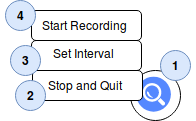
\includegraphics[width=.3\linewidth]{img/ui/ui-lupr-tray}
  \caption{Perancangan antarmuka tampilan \emph{Tray} sistem \emph{Lup
      Recorder}}\label{fig:ui-lupr-tray}
\end{figure}

{\makegapedcells
    \begin{longtable}{|c|L{3.9cm}|L{2cm}|L{6cm}|}
    \caption{Perancangan antarmuka tampilan \emph{Tray} sistem \emph{Lup
        Recorder}}\label{tab:ui-lupr-tray}
    \\\hline
    \thead{No} & \thead{Nama Objek} & \thead{Tipe} & \thead{Keterangan}\\\hline
    %
    1 & \emph{Lup Recorder tray} & Tombol \emph{tray} & Tombol untuk mengakses menu pada sistem \emph{Lup Recorder}. \\\hline
    2 & Tombol ``\emph{Start Recording}'' & Tombol & Tombol memulai merekam tugas. \\\hline
    3 & Tombol ``\emph{Set Interval}'' & Tombol & Tombol mengubah interval rekaman. \\\hline
    4 & Tombol ``Stop and Quit'' & Tombol & Tombol untuk menghentikan perekaman tugas.\\\hline
  \end{longtable}
}

\subsubsection{Perancangan Antarmuka Tampilan Hasil Rekaman Pada Sistem \emph{Lup Viewer}}

Gambar~\ref{fig:ui-lupv-log-view} merupakan rancangan antarmuka
tampilan hasil rekaman pada sistem \emph{Lup Viewer}. Antarmuka ini
merupakan rancangan antarmuka yang digunakan untuk melihat hasil
rekaman. Penjelasan komponen-komponen yang terdapat pada rancangan
tersebut terdapat pada Tabel~\ref{tab:ui-lupv-log-view}.

\begin{figure}[H]
  \centering
  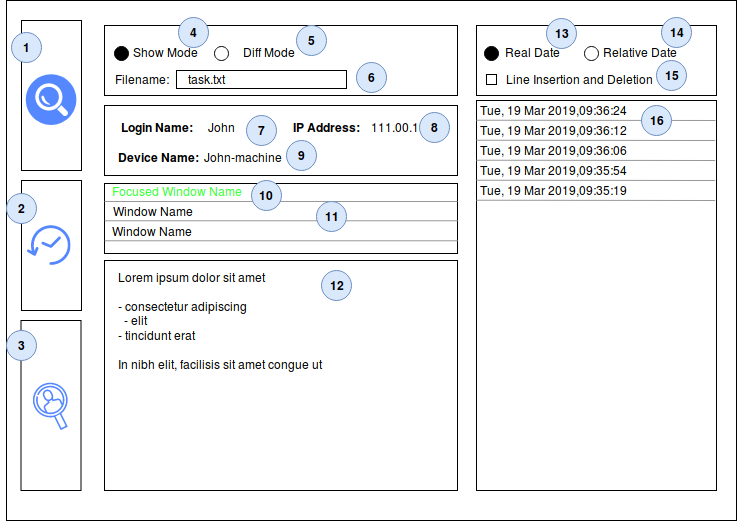
\includegraphics[width=.8\linewidth]{img/ui/ui-lupv-log-view}
  \caption{Perancangan antarmuka tampilan Hasil Rekaman sistem \emph{Lup
      Viewer}}\label{fig:ui-lupv-log-view}
\end{figure}

{\makegapedcells
    \begin{longtable}{|c|L{3.9cm}|L{2cm}|L{6cm}|}
    \caption{Penjelasan antarmuka tampilan Hasil Rekaman sistem \emph{Lup
        Viewer}}\label{tab:ui-lupv-log-view}
    \\\hline
    \thead{No} & \thead{Nama Objek} & \thead{Tipe} & \thead{Keterangan}\\\hline
    %
    1 & Tombol ``\emph{Main View}'' & Tombol & Tombol untuk menuju tampilan utama seluruh daftar rekaman.\\\hline
    2 & Tombol ``\emph{Log View}'' & Tombol & Tombol untuk menuju tampilan hasil rekaman.\\\hline
    3 & Tombol ``\emph{Search View}'' & Tombol & Tombol untuk menuju tampilan analisis hasil rekaman.\\\hline
    4 & Tombol ``\emph{Show Mode}'' & \emph{Radio Button} & \emph{Radio button} untuk mengalihkan mode tampilan rekaman
                                                            berkas ke mode \emph{show}.\\\hline
    5 & Tombol ``\emph{Diff Mode}'' & \emph{Radio Button} & \emph{Radio button} untuk mengalihkan mode tampilan rekaman
                                                            berkas ke mode \emph{diff}.\\\hline
    6 & Tombol ``\emph{Filename}'' & \emph{Combo Box} & \emph{Combo box} untuk memilih nama berkas tugas.\\\hline
    7 & Label ``\emph{Login Name}'' & Label & Label untuk menampilkan nama \emph{login}.\\\hline
    8 & Label ``\emph{Device Name}'' & Label & Label untuk menampilkan nama piranti.\\\hline
    9 & Label ``\emph{IP Address}'' & Label & Label untuk menampilkan alamat \emph{IP}.\\\hline
    10 & Daftar ``\emph{Active Window}'' & \emph{List Widget} & Daftar untuk menampilkan \emph{window}
                                                                yang aktif.\\\hline
    11 & Daftar ``\emph{All Window}'' & \emph{List Widget} & \emph{List widget} untuk menampilkan semua
                                                             \emph{window}.\\\hline
    12 & \emph{Widget} berkas rekaman & \emph{Widget} & \emph{Widget} untuk menampilkan rekaman berkas.\\\hline
    13 & Tombol ``\emph{Real Date}'' & \emph{Radio Button} & \emph{Radio button} untuk mengalihkan mode format waktu
                                                             rekaman ke dalam format waktu \emph{real}.\\\hline
    14 & Tombol ``\emph{Relative Date}'' & \emph{Radio Button} & \emph{Radio button} untuk mengalihkan mode format waktu
                                                                 rekaman ke dalam format waktu relatif.\\\hline
    15 & Tombol ``\emph{Line Insertion and Deletion}'' & \emph{Check Box} & Tombol untuk menampilkan jumlah
                                                                            baris yang ditambah dan dihapus.\\\hline
    16 & Daftar Rekaman & \emph{List Widget} & \emph{List widget} untuk menampilkan daftar rekaman.\\\hline
  \end{longtable}
}

\subsubsection{Perancangan Antarmuka Tampilan \emph{Edit-distance} Tugas Sebelumnya Pada Sistem \emph{Lup Viewer}}

Gambar~\ref{fig:ui-lupv-ed-view} merupakan rancangan antarmuka
tampilan \emph{edit-distance} tugas sebelumnya pada sistem \emph{Lup
  Viewer}. Rancangan antarmuka ini digunakan untuk melihat grafik
\emph{edit-distance} tugas sebelumnya. Penjelasan komponen-komponen
yang terdapat pada rancangan tersebut terdapat pada
Tabel~\ref{tab:ui-lupv-ed-view}.

\begin{figure}[H]
  \centering
  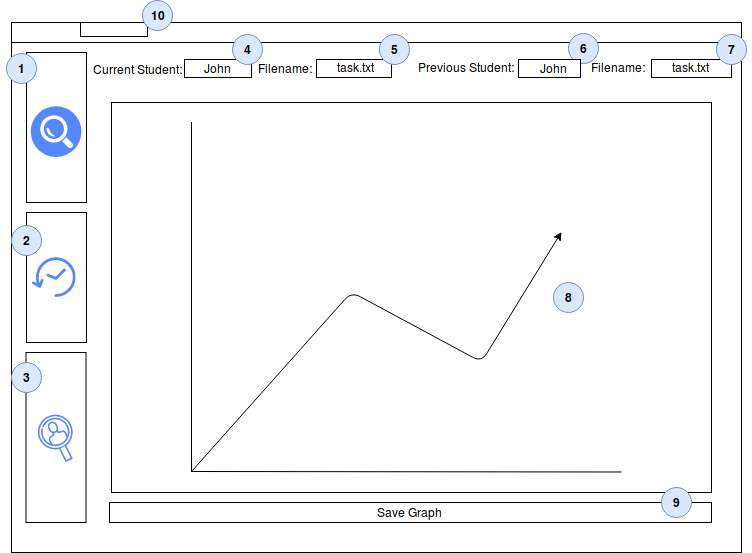
\includegraphics[width=.8\linewidth]{img/ui/ui-lupv-ed-view}
  \caption{Perancangan antarmuka tampilan \emph{Edit-distance} Tugas
    Sebelumnya}\label{fig:ui-lupv-ed-view}
\end{figure}

{\makegapedcells
  \begin{longtable}{|c|L{3.9cm}|L{2cm}|L{6cm}|}
    \caption{Penjelasan antarmuka tampilan \emph{Edit-distance} Tugas
      Sebelumnya}\label{tab:ui-lupv-ed-view}
    \\\hline
    \thead{No} & \thead{Nama Objek} & \thead{Tipe} & \thead{Keterangan}\\\hline
    %
    1 & Tombol ``\emph{Main View}'' & Tombol & Tombol untuk menuju tampilan utama seluruh daftar rekaman.\\\hline
    2 & Tombol ``\emph{Log View}'' & Tombol & Tombol untuk menuju tampilan hasil rekaman.\\\hline
    3 & Tombol ``\emph{Search View}'' & Tombol & Tombol untuk menuju tampilan analisis hasil rekaman.\\\hline
    4 & Tombol ``\emph{Current Student}'' & \emph{Combo Box} & \emph{Combo box} untuk memilih mahasiswa pada tugas saat
                                                               ini.\\\hline
    5 & Tombol ``\emph{Filename}'' & \emph{Combo Box} & \emph{Combo box} untuk memilih berkas tugas saat
                                                               ini.\\\hline
    6 & Tombol ``\emph{Previous Student}'' & \emph{Combo Box} & \emph{Combo box} untuk memilih mahasiswa pada tugas
                                                                sebelumnya.\\\hline
    7 & Tombol ``\emph{Filename}'' & \emph{Combo Box} & \emph{Combo box} untuk memilih mahasiswa pada tugas
                                                        sebelumnya.\\\hline
    8 & \emph{Widget} \emph{Edit-distance} & \emph{Widget} & \emph{Widget} untuk menampilkan grafik
                                                             \emph{edit-distance}.\\\hline
    9 & Tombol ``\emph{Save Graph}'' & Tombol & Tombol untuk menyimpan grafik \emph{edit-distance}.\\\hline
    10 & Tombol ``\emph{Load Edit-distance File}'' & Tombol & Tombol untuk membuka berkas \emph{edit-distance}
                                                              tugas sebelumnya.\\\hline
  \end{longtable}
}


\section{Implementasi Sistem}

Tahapan implementasi sistem merupakan sebuah tahapan yang dilakukan setelah selesainya
proses perancangan sistem. Pada tahapan ini hasil perancangan komponen yang berupa
\emph{pseudocode} diimplementasikan menjadi \emph{working code} menggunakan
bahasa pemrograman \emph{Python} dan bantuan kakas bantu seperti \emph{git}.
Selain itu, Hasil perancangan
antarmuka juga diimplementasikan dengan bantuan \emph{widget toolkit} \emph{Qt}.

\subsection{Spesifikasi Sistem}

Spesifikasi perangkat keras yang digunakan untuk membangun sistem
dipaparkan pada Tabel~\ref{tab:hardware}. Pada Tabel tersebut terdapat
spesifikasi \emph{processor}, \emph{HDD} dan \emph{RAM}. Sementara itu,
spesifikasi perangkat lunak yang digunakan dipaparkan pada
Tabel~\ref{tab:software}, di dalamnya terdapat spesifikasi
sistem operasi, \emph{kernel}, editor dokumentasi, editor pemrograman, dan bahasa
pemrograman.

{\makegapedcells
  \begin{longtable}{|L{4.5cm}|L{6.5cm}|}
   \caption{Spesfikasi perangkat keras} \label{tab:hardware}\\
    \hline
    \thead{Nama Komponen} & \thead{Spesifikasi}\\\hline
    %
    \emph{Processor} & Intel i5-7200U (4) @ 3.1GHz   \\\hline
    \emph{Hard Disk} & 500 GB   \\\hline
    \emph{RAM} & 4 GB    \\\hline
  \end{longtable}
}

{\makegapedcells
  \begin{longtable}{|L{4.5cm}|L{6.5cm}|}
    \caption{Spesfikasi perangkat lunak} \label{tab:software}\\
    \hline
    \thead{Nama Komponen} & \thead{Spesifikasi}\\\hline
    %
    Sistem Operasi & Debian GNU/Linux 9.6 (stretch) x86\_64 \\\hline
    \emph{Kernel} & Kernel: 4.9.0-6-amd64    \\\hline
    Editor Dokumentasi & GNU Emacs 26.1  \\\hline
    Editor Pemrograman & GNU Emacs 26.1  \\\hline
    Bahasa Pemrograman & Python 3.6.4    \\\hline
  \end{longtable}
}

\subsection{Implementasi Kode Program}

Pada tahapan implementasi kode program. Hasil rancangan komponen
sistem pada tahapan perancangan komponen sistem diimplementasikan
menjadi \emph{working code} dengan bahasa pemrograman \emph{Python}.
Subbab 5.2.2.1 hingga 5.2.2.3 memaparkan
implementasi dari tiga sampel \emph{class} pada tahapan perancangan
komponen sebelumnya, yaitu \emph{class} \emph{Controller} pada sistem
\emph{Lup Recorder}, \emph{class} \emph{LogController} pada sistem
\emph{Lup Viewer}, dan \emph{class} \emph{SearchController} pada
sistem \emph{Lup Viewer}.

\subsubsection{Implementasi Kode Program \emph{Class} \emph{Controller} Pada Sistem \emph{Lup Recorder}}

Pada Tabel Kode~\ref{code:get_all_windows} dipaparkan \emph{source
  code} \emph{get\_all\_windows}. \emph{Source code}
\emph{get\_all\_windows} mengimplementasikan hasil rancangan
\emph{pseudocode} pada tahapan sebelumnya. \emph{Source code}
\emph{get\_all\_windows} mengambil seluruh informasi \emph{window}
yang kemudian melakukan filter dan hanya mengembalikan nama
\emph{window} saja.

\par\null\par
\begin{code}
\begin{ignasicblock}[title=get\_all\_windows,minted language=Python]
def get_all_windows(self):
  all_windows = ""
  all_windows_proc = Popen(["wmctrl", "-l"], stdout=PIPE)
  all_windows_dirty, err = all_windows_proc.communicate()
  if all_windows_dirty:
    all_windows_dirty = all_windows_dirty.splitlines()
    for line in all_windows_dirty:
      windows_name = line.split(None, 3)[-1].decode()
      all_windows += "{}\n".format(windows_name)
  return all_windows
\end{ignasicblock}
    \captionof{listing}{Source code \emph{function get\_all\_windows}}\label{code:get_all_windows}
\end{code}

\subsubsection{Implementasi Kode Program \emph{Class} \emph{LogController} Pada Sistem
  \emph{Lup Viewer}}

Pada Tabel Kode~\ref{code:populate_logs} dipaparkan \emph{source code}
\emph{populate\_log}. \emph{Source code} \emph{populate\_log}
mengimplementasikan hasil rancangan \emph{pseudocode} pada tahapan
sebelumnya. \emph{Source code} \emph{populate\_log} membaca seluruh
rekaman mahasiswa, dari setiap rekaman diambil nilai-nilai yang
dibutuhkan di antaranya adalah waktu rekaman, baris yang ditambah, dan
baris yang dihapus.

\par\null\par
\begin{code}
\begin{ignasicblock}[title=populate\_logs,minted language=Python]
def populate_logs(self, selected_file=None):
  student_records = self._log_model.student_records

  for record in student_records:
    relative_time = self._main_ctrl.relativize_datetime(
      record.committed_datetime
    )
    time_format = "{:%a, %d %b %Y, %H:%M:%S}"
    time = time_format.format(record.committed_datetime)
    sha = record.hexsha
    insertions = 0
    deletions = 0

    if selected_file:
      if self._log_model.is_exists(selected_file, sha):
        insertions = record.stats.files[selected_file]["insertions"]
        deletions = record.stats.files[selected_file]["deletions"]

    log = dict(
      relative_time=relative_time,
      time=time,
      sha=sha,
      insertions=insertions,
      deletions=deletions,
    )
    yield log
\end{ignasicblock}
    \captionof{listing}{Source code \emph{function populate\_logs}}\label{code:populate_logs}
\end{code}

\subsubsection{Implementasi Kode Program \emph{Class} \emph{SearchController} Pada Sistem
  \emph{Lup Viewer}}

Pada Tabel Kode~\ref{code:populate_logs} dipaparkan \emph{source code}
\emph{construct\_ed\_graph\_path}. \emph{Source code}
\emph{construct\_ed\_graph\_path} mengimplementasikan hasil rancangan
\emph{pseudocode} pada tahapan sebelumnya. \emph{Source code}
\emph{construct\_ed\_graph\_path} membangun \emph{path} untuk nama
grafik \emph{edit-distance} yang disimpan. \emph{Path} tersebut
mengikuti jumlah mahasiswa yang ada. Jika terdapat lebih dari satu
mahasiswa, maka diberikan ``\_'' sebagai penghubung nama antar
mahasiswa.

\par\null\par
\begin{code}
\begin{ignasicblock}[title=construct\_ed\_graph\_path,minted language=Python]
def construct_ed_graph_path(self, *args):
  record_path = self._main_model.record_path

  if len(args) == 1:
    graph_fmt = "{}.png".format(args[0])
  else:
    names = "_".join(args)
    graph_fmt = "{}.png".format(names)

  graph_path = join(record_path, "lupv-notes", graph_fmt)
  return graph_path
\end{ignasicblock}
  \captionof{listing}{\emph{Source code} \emph{function construct\_ed\_graph\_path}}\label{code:load_data}
\end{code}

\subsection{Implementasi Antarmuka}

Pada Tahapan ini, hasil rancangan antarmuka pada tahapan sebelumnya
diimplementasikan menggunakan \emph{widget toolkit} \emph{Qt}.
Tiga sampel implementasi antarmuka yang dipaparkan adalah antarmuka tampilan
\emph{tray} pada sistem \emph{Lup Recorder} pada
Gambar~\ref{fig:ss-lupr-tray}, antarmuka tampilan hasil rekaman pada
sistem \emph{Lup Viewer} pada Gambar~\ref{fig:ss-lupv-log-view}, dan
antarmuka tampilan \emph{edit-distance} tugas sebelumnya pada sistem
\emph{Lup Viewer} pada Gambar~\ref{fig:ss-lupv-ed-view}.

\subsubsection{Implementasi Antarmuka Tampilan \emph{Tray} Pada Sistem \emph{Lup Recorder}}

Gambar~\ref{fig:ss-lupr-tray} merupakan implementasi antarmuka
tampilan \emph{tray} pada sistem \emph{Lup Recorder}. Implementasi ini
dibangun berlandaskan tahapan perancangan antarmuka
sebelumnya. Antarmuka ini merupakan rancangan antarmuka utama pada
sistem \emph{Lup Recoder} dan digunakan untuk mengakses seluruh menu
utama sistem \emph{Lup Recorder}.

\begin{figure}[H]
  \centering
  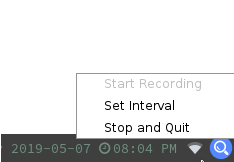
\includegraphics[width=.5\linewidth]{img/ui/ss-lupr-tray}
  \caption{Implementasi antarmuka tampilan \emph{Tray} pada sistem
    \emph{Lup Recorder}}\label{fig:ss-lupr-tray}
\end{figure}

\subsubsection{Implementasi Antarmuka Tampilan Hasil Rekaman Pada Sistem \emph{Lup Viewer}}

Gambar~\ref{fig:ss-lupv-log-view} merupakan implementasi antarmuka
tampilan hasil rekaman pada sistem \emph{Lup Viewer}. Implementasi ini
dibangun berlandaskan tahapan perancangan antarmuka
sebelumnya. Antarmuka ini merupakan rancangan antarmuka yang digunakan
untuk melihat hasil rekaman.

\begin{figure}[tph]
  \centering
  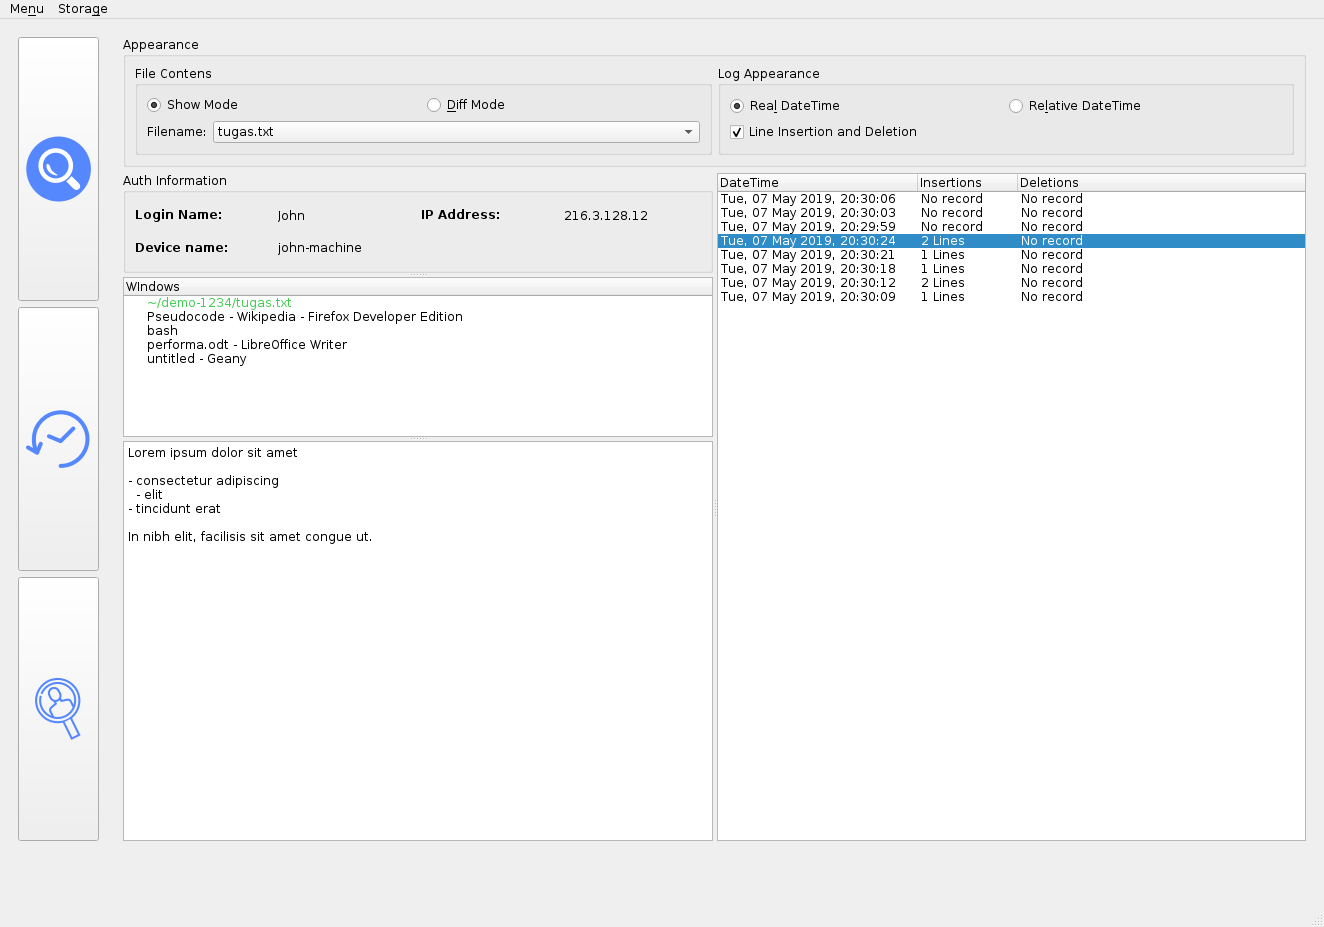
\includegraphics[width=.9\linewidth]{img/ui/ss-lupv-log-view}
  \caption{Implementasi antarmuka tampilan Hasil Rekaman pada sistem \emph{Lup
      Viewer}}\label{fig:ss-lupv-log-view}
\end{figure}

\subsubsection{Perancangan Antarmuka Tampilan \emph{Edit-distance} Tugas Sebelumnya Pada Sistem \emph{Lup Viewer}}

Gambar~\ref{fig:ss-lupv-ed-view} merupakan implementasi antarmuka
tampilan \emph{edit-distance} tugas sebelumnya pada sistem \emph{Lup
  Viewer}. Implementasi ini dibangun berlandaskan tahapan perancangan
antarmuka sebelumnya. Antarmuka ini digunakan untuk melihat grafik
\emph{edit-distance} tugas sebelumnya.

\begin{figure}[tph]
  \centering
  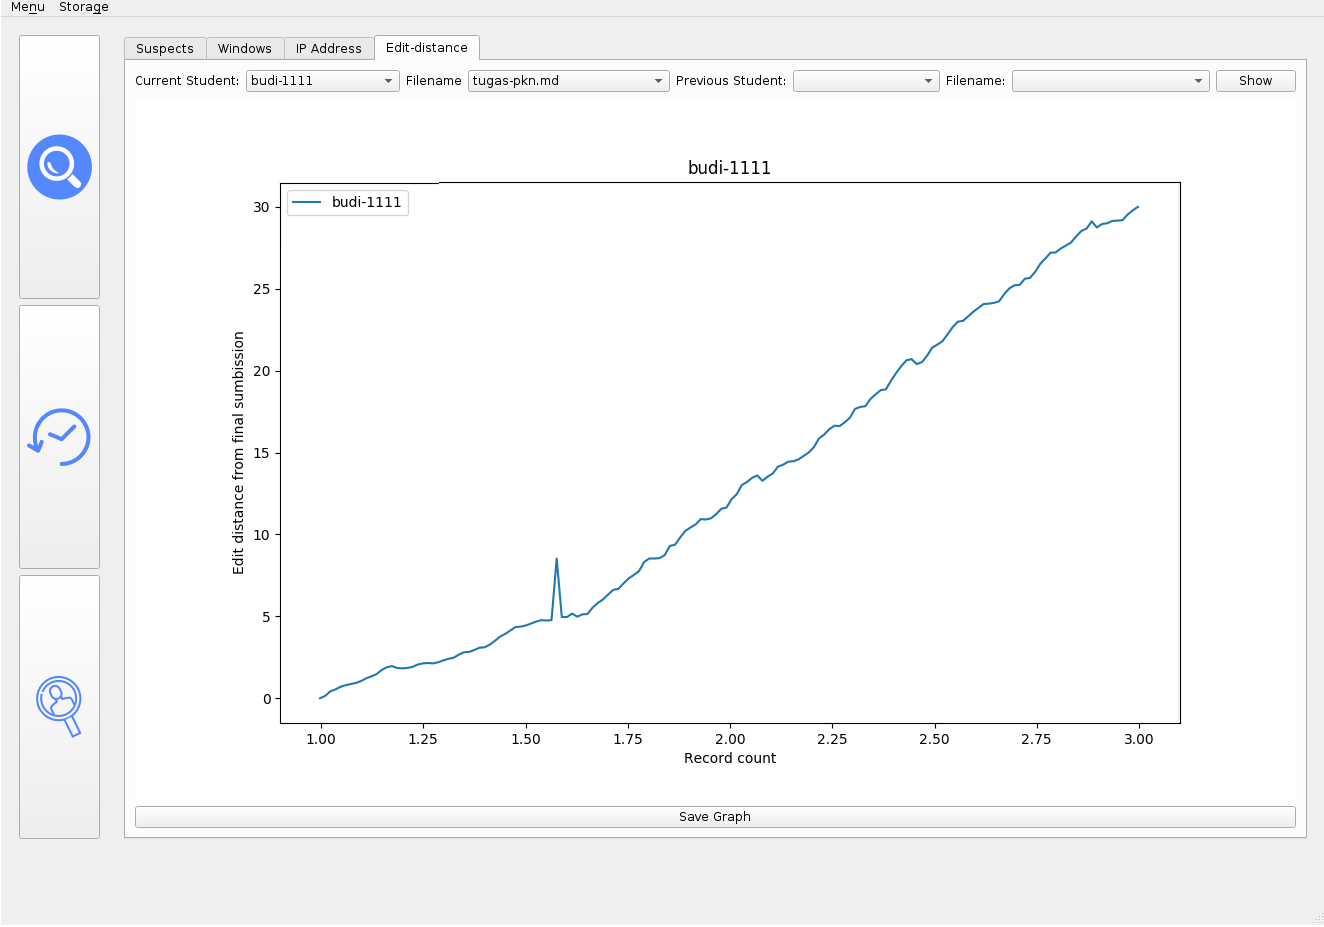
\includegraphics[width=.9\linewidth]{img/ui/ss-lupv-ed-view}
  \caption{Perancangan antarmuka tampilan \emph{Edit-distance} Tugas Sebelumnya
    pada sistem \emph{Lup Viewer}}\label{fig:ss-lupv-ed-view}
\end{figure}


%%% Local Variables:
%%% coding: utf-8
%%% mode: latex
%%% TeX-engine: xetex
%%% TeX-master: "skripsi"
%%% ispell-local-dictionary: "id"
%%% End:
